\section{Результаты}
Для удобной работы с реальными изображениями мною был переделан формат класстеров. По условию кластер представляет собой набор пикселей.
Для удобного ввода я представил кластер в виде прямоугольника и подавал на вход лишь координаты левого верхнего и правого нижнего углов прямоугольника.

\textbf{Примеры работы программы:}
\begin{center}


\includegraphics[width=.49\textwidth]{1}\hfill
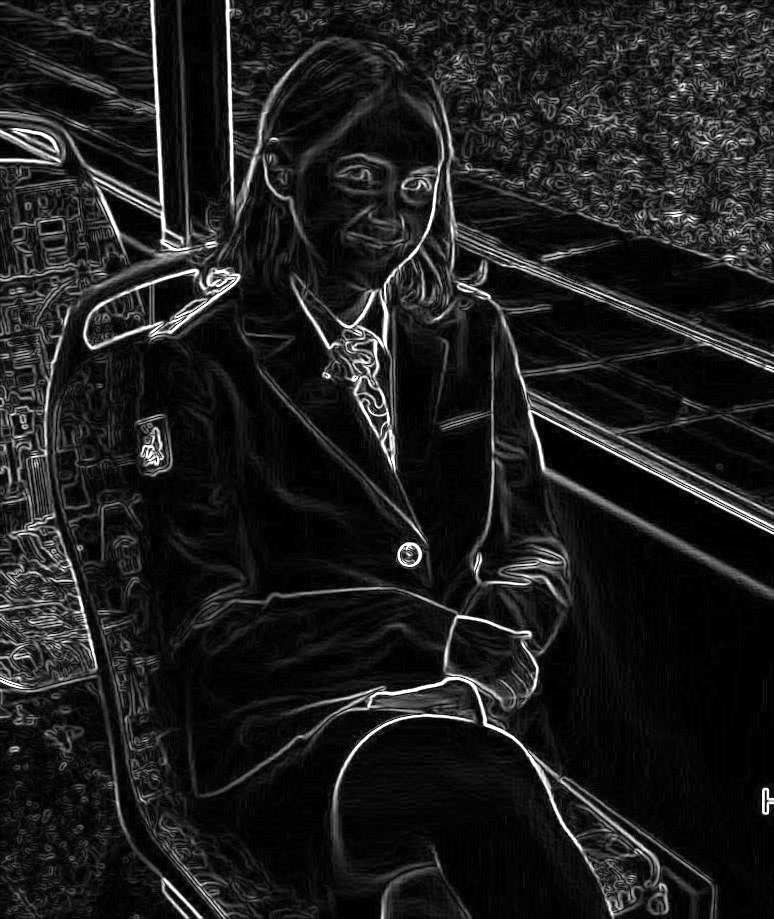
\includegraphics[width=.49\textwidth]{1_out}

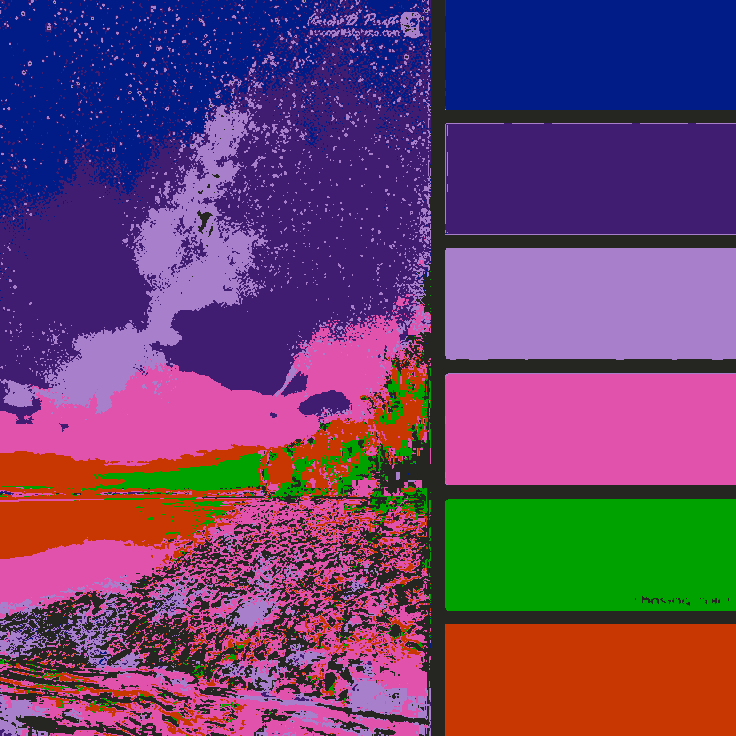
\includegraphics[width=.49\textwidth]{2}\hfill
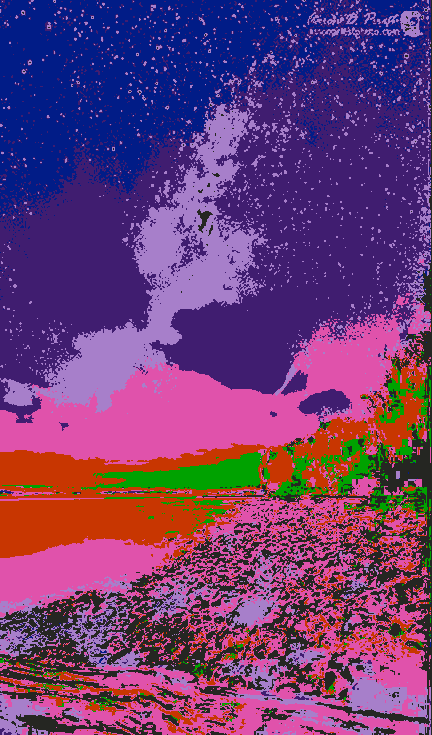
\includegraphics[width=.49\textwidth]{2_out}

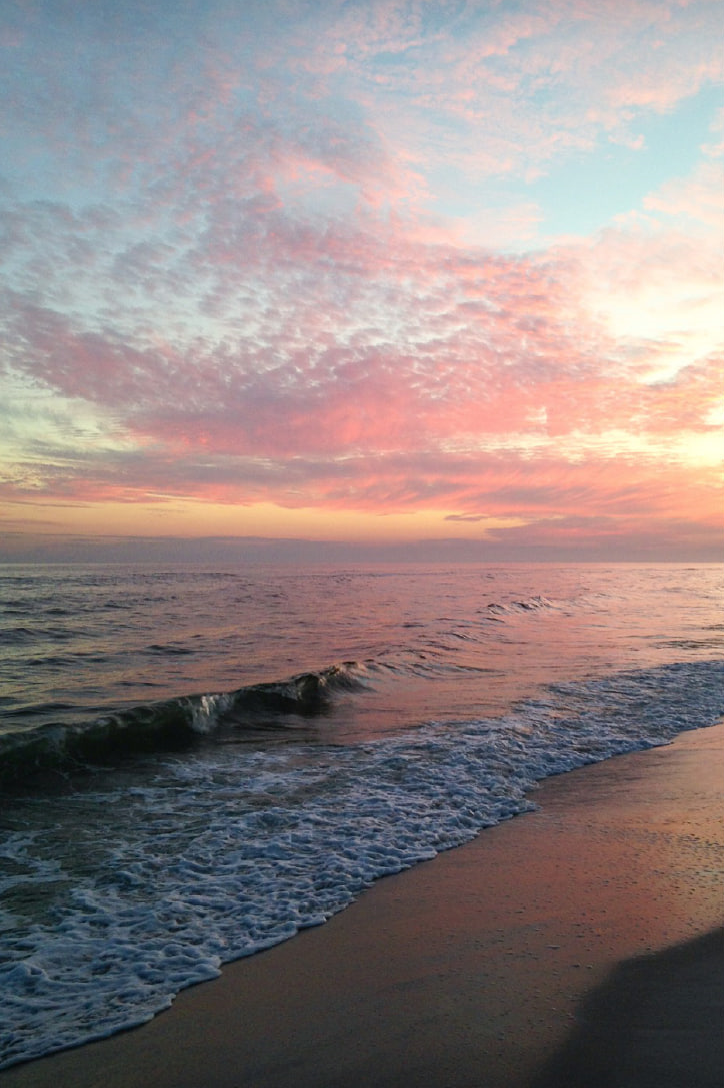
\includegraphics[width=.49\textwidth]{3}\hfill

\includegraphics[width=.49\textwidth]{3_out}

\end{center}

В качестве тестовых данных было взято квадратное изображение заданного размера. Пиксели генерировались с помощью генератора псевдослучайных чисел.

\textbf{Сравнение времени работы}

\makebox[\textwidth][c]{
\small
\begin{tabular}{|l*{8}{|r}|}
\hline
\textbf{Размер теста} & 100$\times$100 & 500$\times$500 & 1000$\times$1000 & 1000$\times$1000 & 2000$\times$2000 & 2000$\times$2000 & 5000$\times$5000 & 5000$\times$5000 \\
\textbf{Число классов} & \multicolumn{1}{c|}{10} & \multicolumn{1}{c|}{10} & \multicolumn{1}{c|}{10} & \multicolumn{1}{c|}{32} & \multicolumn{1}{c|}{10} & \multicolumn{1}{c|}{32} & \multicolumn{1}{c|}{10} & \multicolumn{1}{c|}{32} \\
\hline
\hline
\textbf{Конфигурация} & \multicolumn{8}{c|}{\textbf{Время выполнения, мс}} \\
\hline
CPU        &   9.1379 & 189.2646 & 529.117 & 1545.433 & 1937.266 & 5923.956 & 11940.333 & 36821.500 \\
\hline
1, 32      &   1.4703 &  38.0822 & 152.122 &  442.399 &  608.409 & 1769.516 &  3802.423 & 11058.966 \\
\hline
32, 32     &   0.1618 &   3.4147 &  13.548 &   40.965 &   54.131 &  164.102 &   338.453 &  1028.226 \\
\hline
64, 64     &   0.1383 &   2.7711 &  11.035 &   34.528 &   44.074 &  138.093 &   275.482 &   862.861 \\
\hline
128, 128   &   0.1385 &   2.6698 &  10.624 &   33.326 &   42.452 &  133.250 &   265.203 &   832.737 \\
\hline
256, 256   &   0.1378 &   2.6618 &  10.618 &   33.315 &   42.408 &  133.211 &   264.936 &   832.471 \\
\hline
512, 512   &   0.1647 &   2.7680 &  10.757 &   33.754 &   42.873 &  134.950 &   267.780 &   843.309 \\
\hline
1024, 1024 &   0.2754 &   2.9208 &  11.234 &   34.477 &   43.730 &  136.688 &   271.044 &   852.250 \\
\hline
\end{tabular}
}
\pagebreak